\section{Durchführung}
\label{sec:Durchführung}
Zu Beginn werden die verwendeten Stäbe ausgemessen. Hierbei wird die Länge, der
Durchmesser sowie das Gewicht notiert.
In folgender Abbildung \ref{fig:aufbau} ist der Aufbau des Versuches schematisch dargestellt.
\begin{figure}[H]
  \centering
  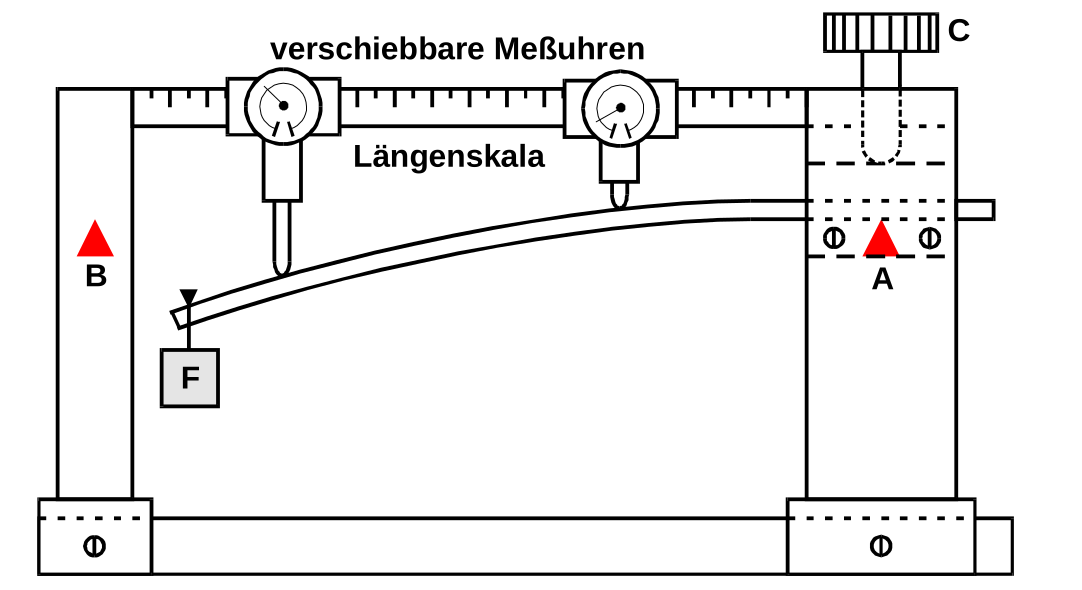
\includegraphics[scale=0.4]{content/versuchsaufbau.png}
  \caption{Schematischer Aufbau der verwendeten Apparatur.}
  \label{fig:aufbau}
\end{figure}
\noindent
Hierbei können die Probenstäbe entweder einseitig oder beidseitig eingespannt
werden. Es gibt zwei Auflagepunkte, von denen der Auflagepunkt \textbf{A} eine
Spannvorrichtung besitzt, um den Stab einseitig einspannen zu können.
Die Gewichte werden bei einseitiger Einspannung an das nicht eingespannte
Ende gehängt, bei beidseitiger Einspannung wird das Gewicht bei $x = L/2$ befestigt.
Die Durchbiegung des Stabes kann mithilfe der beiden beweglichen Messuhren ermittelt werden.
Die Messuhren besitzen eine Mikrometer-Skala und werden auf einer Millimeter-Skala positioniert.
Die Gewichte werden so gewählt, dass die maximale Durchbiegung zwischen $\SI{3}{\milli\meter}$ bis
$\SI{7}{\milli\meter}$ liegt.

\subsection{Einseitige Einspannung des Stabes}
Die im Folgenden beschriebene Messung wird einmal für einen runden und einmal für
einen eckigen Stab durchgeführt. Der Stab wird einseitig in die in Abbildung \ref{fig:aufbau}
gezeigte Apparatur eingespannt. Die eine Messuhr wird auf den Anfang der Messskala
geschoben, die andere wird hier nicht verwendet. Das Gewicht wird nach Messung der
Durchbiegung in der Ruhelage angehängt. Nun wird die Messuhr in regelmässigen Abständen
an der Skala entlang bewegt und die Messwerte werden aufgenommen. 

\subsection{Beidseitige Einspannung des Stabes}
Die im Folgenden beschriebene Messung wird mit einem runden Stab durchgeführt.
In der in Abbildung \ref{fig:aufbau} beschriebenen Apparatur wird der Stab an den
Punkten \textbf{A} und \textbf{B} eingespannt. Die eine Messuhr wird erneut auf den
Anfang der Skala geschoben, die andere auf das Ende der Skala. Die Messuhren werden
in regelmässigen Abständen auf die Mitte des Stabes zubewegt.
